\documentclass[a4paper,12pt]{report}
\usepackage[utf8x]{inputenc}
\usepackage[francais]{babel}
\usepackage[svgnames]{xcolor}
\usepackage{varioref}
\usepackage{textcomp}
\usepackage{graphicx}
\usepackage{tikz}
\usepackage{url}
\usepackage{ifthen}
\usepackage{xstring}
\usepackage{calc}
\usepackage{pgfopts}
\usepackage{titlesec}
\usepackage{listings}
\usepackage{hyperref}
\hypersetup{colorlinks=true, linkcolor=black}
\usepackage{color}

\lstset{ %
  language=C++,                     % the language of the code
  basicstyle=\footnotesize,       % the size of the fonts that are used for the code
  numbers=left,                   % where to put the line-numbers
  numberstyle=\tiny\color{gray},  % the style that is used for the line-numbers
  stepnumber=1,                   % the step between two line-numbers. If it's 1, each line
                                  % will be numbered
  numbersep=5pt,                  % how far the line-numbers are from the code
  backgroundcolor=\color{white},  % choose the background color. You must add \usepackage{color}
  showspaces=false,               % show spaces adding particular underscores
  showstringspaces=false,         % underline spaces within strings
  showtabs=false,                 % show tabs within strings adding particular underscores
  frame=single,                   % adds a frame around the code
  rulecolor=\color{black},        % if not set, the frame-color may be changed on line-breaks within not-black text (e.g. commens (green here))
  tabsize=2,                      % sets default tabsize to 2 spaces
  captionpos=b,                   % sets the caption-position to bottom
  breaklines=true,                % sets automatic line breaking
  breakatwhitespace=false,        % sets if automatic breaks should only happen at whitespace
  title=\lstname,                 % show the filename of files included with \lstinputlisting;
                                  % also try caption instead of title
  keywordstyle=\color{blue},      % keyword style
  commentstyle=\color{magenta},   % comment style
  stringstyle=\color{red},      % string literal style
  escapeinside={\%*}{*)},         % if you want to add a comment within your code
  morekeywords={*,...}            % if you want to add more keywords to the set
} 

\bibliographystyle{plain}
\frenchbsetup{StandardLists=true}

%%%%%%%%%%%%%%%%%%%%%%%%%%%%%%%%%%%%%%% PDF INFO 
%%%%%%%%%%%%%%%%%%%%%%%%%%%%%%%%%%%%%%%%%%%%%%%%
\hypersetup{
	pdfauthor   = {Erwan Douaille et Yoan Miranda},
	pdftitle    = {Rapport de Projet Individuel},
	pdfsubject  = {Kinect interraction},
	pdfkeywords = {Kinect Erwan Douaille Yoan Miranda Lille},
	pdfcreator  = {PDFLaTeX},
	pdfproducer = {PDFLaTeX}
}
%%%%%%%%%%%%%%%%%%%%%%%%%%%%%%%%%%%%%%%%%%%%%%%%

\author{Douaille Erwan et Yoan Miranda}
\title{}
\titleformat{\chapter}[hang]{\bf\huge}{\thechapter}{2pc}{}


\begin{document}

\makeatletter
\begin{titlepage}
\centering
\vspace{-10em}
{\LARGE \textbf{\textsc{Rapport de Projet RVI}}}\\
\vspace{3em}

\includegraphics[scale=0.6]{image/thalassa.png}\\
\vspace{3em}
{\LARGE \textsc{Projet Thalassa: simulation de plongée sous-marine}}\\

\vspace{8em}
Par\\
\vspace{1em}
{\LARGE \@author}\\

\vspace{2em}



\begin{tikzpicture}[remember picture,overlay]

\node [below left,xshift=-1cm, yshift=4cm] at (current page.south east){
\includegraphics[scale=0.6]{image/ustl1.png}};

\end{tikzpicture}
\end{titlepage}
\makeatother

\sloppy	

\chapter*{Remerciements}

Nous souhaitons remercier l'ensemble de l'équipe MINT pour son accueil et le prêt de matériel nécessaire à la réalisation de notre projet, cf Kinect.

Nous souhaitons remercier plus particullièrement Patricia Plénacoste pour la correction apporté à notre rapport ainsi que Samuel Degrande pour la correction de notre rapport, son suivis de projet ainsi que pour les conseils et aide technique nécessaire à l'implémentation de la Kinect dans WabinPaint.

Nous remercions également Claire Bieri pour la relecture de notre rapport ainsi que Daouiya Khadar pour avoir testé notre projet et nous avoir fournie le feedback nécessaire pour le réglage du filtre.

\newpage


\chapter*{Résumé}

TODO ?


\tableofcontents
\thispagestyle{empty}
\newpage
\setcounter{page}{1} 

%%%%%%%%%%%%%%%%%%%%%%%%%%%%%%%%%%%%%%% contenu futur
\chapter{Introduction}

Avec la montée en puissance de calcul des processeurs graphiques (GPU) le monde de l'imagerie a ces vingts dernières années énormément évolué. L'une de ces évolutions est l'apparition d'écran large. Les écrans larges d'il y a dix ans, qui représentent des écrans 21"\cite{Czerwinski:2006:LDR:1125451.1125471}, sont aujourd'hui très courants dans le milieu des ordinateurs de bureau et sont souvent utilisés en multi-monitoring. Notre définition d'écrans larges correspond à des murs, soit des écrans par exemple de quatre mètres de large pour deux mètres de haut. Alors que Czerwinsky et al.\cite{czerwinski2003toward} démontrent que les écrans d'une vingtaine de pouces apportent un gain de confort, de performance et de précision dans l'utilisation des ordinateurs, on remarque que pour des écrans larges faisant la taille d'un mur ce constat n'est plus valable. Comme visible dans de nombreuses études \cite{Schmidt:2013:SEP:2470654.2466227, Vogel:2004:IPA:1029632.1029656, jakobsen2013information} les écrans larges apportent de nouvelles questions comme, comment interagir avec des grands écrans, comment afficher une image pour différents points de vue, ou encore comment apporter un confort visuel aux personnes ayant des troubles visuels tout en utilisant de grands écrans. L'interaction et l'appréhension de l'image sur écran géant sont différentes de ce que l'on rencontre sur des écrans classiques d'une vingtaine de pouces.

\section{Problématique} 

Deux problèmes en particulier apparaissent lors de l'utilisation d'écrans géants. L'un étant que lorsque l'utilisateur est proche de l'écran un effet de perspective apparaît ce qui pose problème pour interagir avec ce qui est situé aux bords de l'écran. Le second problème est lors d'une interaction distante, à cause de la grande densité de pixel que l'écran fournit, il est difficile de voir tout les détails de l'écran ce qui apporte une difficulté et une imprécision dans l'interaction.

Pour répondre à ces deux problèmes, deux solutions sont envisageables. La première est de travailler sur la partie interaction pour permettre d'aider l'utilisateur à mieux interagir avec ces grands écrans. La seconde solution est de déformer l'image pour obtenir une taille d'affichage cohérente avec les capacités d'interaction. Dans cette étude nous travaillerons sur la seconde solution qui est la déformation d'image.

Nous verrons donc comment correctement déformer l'image en tenant compte de la position de l'utilisateur face à l'écran pour lui fournir la meilleure interaction possible.


%
%\chapter{Introduction}
%
%Une anamorphose est une déformation réversible d'une image à l'aide d'un système optique, tel un miroir courbe, ou un procédé mathématique. Le but de ce projet est d'étudier l’anamorphose dite dynamique qui fut introduite pour la première fois en 2007 par Solina, F. et Batagelj, B \cite{dynamicAnamorphosis}. L’aspect dynamique de l’anamorphose consiste à ne pas appliquer une déformation statique de l’image, mais à déformer l’image en temps réel en tenant compte de paramètres tels que la position de l’utilisateur face à l’image. 
%
%\section{Contexte}
%
%Ce projet, se basant sur l’anamorphose dynamique de Solina, F. et Batagelj, B \cite{solina2007dynamic}, consiste à appliquer l'anamorphose à un système d'exploitation autrement dit, à un ordinateur avec lequel l’utilisateur peut interagir. Dans notre cas, l'ordinateur utilise un écran géant de 2 mètres de haut sur 4 mètres de largeur. Face à un tel écran l'utilisateur voit apparaître un effet de perspective lorsque celui-ci est très proche de l’écran et qu’il souhaite regarder les éléments qui sont présents au bord de l’écran.
%
%\section{Problématique} 
%
%L'objectif principal de ce projet est de pouvoir apporter un confort visuel à l'utilisateur. Cet objectif vise à corriger l'effet de perspective qui pourrait apparaître sur des écrans géants ou encore apporter une facilité visuelle d'interaction avec ce type d'écran qui possède une densité de pixel par pouce élevé et pour lesquels les systèmes d'exploitation moderne ne sont aujourd'hui pas adaptés. 

\section{Plan du projet}

Dans un premier temps, un état de l'art présente ce qui a déjà été réalisé autour de la déformation d'image ainsi que des techniques pour apporter du confort visuel. Une seconde partie concerne les contributions apportées par cette étude: proposition d'un cadre logiciel permettant la déformation totale ou partielle de l'image tout en conservant les propriétés d'interaction,  et la mise en œuvre sur deux cas d'usage. Ce rapport se finit par une conclusion et des perspectives sur la suite de ce travail sont proposées.
\chapter{Contexte}

Ce projet s'insère dans une collaboration entre l'équipe MINT du LIFL et la Fondation Hopale, visant à mettre à disposition du Centre Jacques Calvé (à Berck-sur-Mer) des applications utilisant les technologies de la Réalité Virtuelle dans un but de rééducation fonctionnelle.

\section{Fondation Hopale}

La Fondation Hopale est un établissement reconnu d'utilité publique. Elle représente 1100 lits et places dans la région Nord/Pas-de-Calais et un effectif de 2500 personnes dans les secteurs sanitaire ESPIC (Etablissement de Santé Privé d'Intérêt Collectif) et Médico-social. Son activité hospitalière est essentiellement orientée vers les pathologies de l’appareil locomoteur, tant en court séjour (chirurgie orthopédique, rhumatologie, neurologie, prise en charge de la douleur), qu’en soins de suite et de réadaptation (département des blessés crâniens, traumatisés médullaires, polytraumatisés et autres prises en charge spécialisées lourdes). Son activité de rééducation dispose avec le Centre Jacques Calvé du plus grand plateau technique de France.

\section{Équipe MINT LIFL}

L'équipe MINT travaille sur l'interaction homme machine. L'interaction gestuelle est leurs sujet d'étude principal, c'est à dire l'utilisation du geste dans une interaction homme machine. Le geste est définit comme un mouvement d'une partie du corps pour exprimer une idée ou un sens, souvent réalisé avec les mains ou la tête. Cette interaction peut se traduire par la pression d'un doigt sur une surface tactile ou encore une information de position.

\chapter{Projet Kinect pour une application de peinture à main levée}


\section{Présentation}

Ce projet porte sur l'adaptation d'une application existante (peinture à main levée) qui utilise comme dispositif d'interaction un système de motion capture ARTrack d'un coût élevé. L'objectif est de permettre une interaction par Kinect.

Kinect est l'outil développé par l'entreprise \textit{PrimeSense} et popularisé par \textit{Microsoft}  avec la Xbox 360. Il s'agit d'une caméra permettant de contrôler avec son corps, ou par commande vocale des applications, jeux, etc. PrimeSense fournit des codes Samples permettant d'utiliser les outils de détection de mouvements, de squelettes et de communication vocale. La détection du squelette sera utilisé et plus particullièrement la détection des mains pour pouvoir interagir avec WabinPaint et permettre à l'utilisateur de dessiner.

L'ajout du contrôle via Kinect est pertinent puisqu'il s'agit d'un outil grand public et à faible coût, contrairement aux outils déjà implémenté dans WabinPaint. De plus l'outil Kinect simplifie la mise en place du dispositif puisque aucun réglage n'est nécessaire contrairement aux dispositifs infrarouges qui nécessitent une calibration et un placement défini de l'utilisateur.

L'utilisation de Kinect a pour but la rééducation fonctionnelle. L'application sera utilisée pour des patients atteints d'héminégligence accompagnée de faibles troubles moteurs. L'héminégligence signifie qu'ils ne percoivent qu'une partie de leur environnement et sont donc, par exemple, dans l'incapacité de dessiner la totalité d'un objet. WabinPaint utilisant Kinect, permettra à ces patients de dessiner tout en utilisant leurs gestes, ce qui favorise leurs rééducation fonctionelle.

Le signal produit par la Kinect est fortement bruité (il s'apparente à un tremblement). Un traitement du signal sera effectué grâce au \textit{One Euro Filter}.

\section{WabinPaint}

WabinPaint est une application de dessin développée par l'équipe de recherche MINT comme démonstrateur de ses travaux sur les interactions à mains libres.

Cette application permet à un utilisateur d'utiliser plusieurs méthodes de tracking différentes comme par exemple, une souris, des trackers infrarouges, etc. Wabinpaint permet de dessiner dans un canvas en trois dimensions et propose une rotation du dessin pour visualiser la profondeur.

Plusieurs options de dessin sont également disponibles telles que:
\begin{itemize}
	\item couleur du pinceaux
	\item épaisseur du pinceaux
	\item rotation du canvas
	\item effacement du canvas
\end{itemize}

Voici un rendu de l'application: 
\begin{figure}[!ht]
	\center
	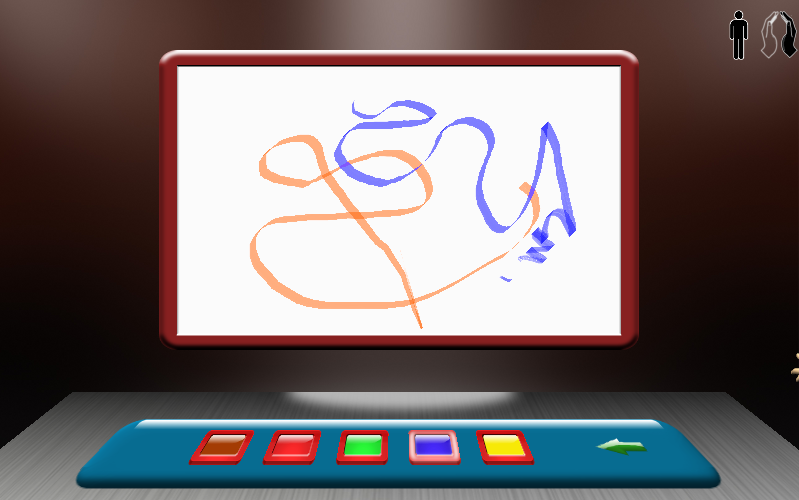
\includegraphics[scale=0.45]{image/wabinpaint.png}
	\caption{Screenshot de WabinPaint}
\end{figure}

\newpage

\section{Objectif}

L'objectif de ce projet est de comprendre comment Kinect fonctionne, d'appliquer des traitements, des lissages sur les cordonnées des mains dans un plan en trois dimensions, pour que l'utilisateur puisse dessiner.

Le projet comportera trois parties distinctes qui sont:
\begin{itemize}
\item Traitement des données Kinect et génération du squelette
\item Récupération de la position des mains et intégration dans WabinPaint
\item Traitement du bruit des positions 
\end{itemize}


\section{Méthodologie de gestion de projet}
Pour concevoir une base logicielle solide et avoir des points de vues différents nous avons (Erwan Douaille \&\ Yoan Miranda) pair-programmé. Le code source du projet est disponible sur la forge de développement de l'équipe MINT.
\chapter{Analyse de l'existant}

WabinPaint est un logiciel utilisant la librairie Clutter. Voici un descriptif plus technique de WabinPaint, ce qui permettra de modéliser une solution pour l'implémentation de la Kinect.

\section{Clutter}

	Clutter est une bibliothèque logicielle permettant la création rapide d'interfaces graphiques visuellement riches et animées. C'est un projet libre (licence GNU LGPL) et multiplate-forme. Clutter est basée sur glib, librairie de l'écosystème Gnome.
	
	Clutter ne gère en périphérique d'entrée que la souris. Cependant il est possible d'associer des données (avec Kinect, la position des mains) à la structure de données représentant la souris. WabinPaint possède déjà une classe qui permettra à notre implémentation Kinect de faire ces opérations, de convertir les positions en événement souris. Cette classe se nomme GenericTracker et est déjà utilisé par les trackers "réels" ART et Vicon. Son utilisation sera détaille dans le chapitre Kinect.
	
\section{Choix techniques}

	OpenNI est une librairie permettant de récupérer la position des mains. Une description de OpenNI plus approfondie est disponible dans le chapitre Kinect.
	
	Pour fonctionner OpenNI nécessite de créer une boucle de traitement pour continuellement fournir la position des mains. Pour cette raison et pour ne pas bloquer la boucle de la glib, il est nécessaire d'éxécuter OpenNI dans un thread différent.
	
	À ce problème s'offre deux possibilités, utiliser un thread glib, ou utiliser une application externe (un serveur) et intégrer une partie client en utilisant
     une fonction "idle" dans WabinPaint. C'est cette 2\up{ème} solution qui
     a été choisie pour les deux trackers déjà implémentés dans WabinPaint. L'implémentation de la Kinect sera similaire.
     
 \section{Mise en œuvre}

Pour nous aider au maximum à identifier les différentes parties du projet, nous avons défini plusieurs briques (composantes) visibles ci-dessous:

\begin{figure}[!ht]
	\center
	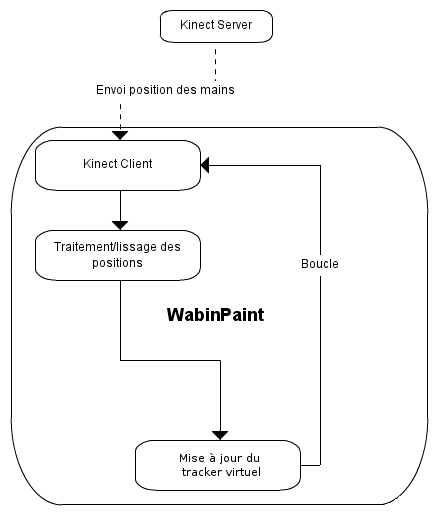
\includegraphics[scale=0.5]{image/plan.png}
	\caption{Composantes à réaliser}
\end{figure}

Sur ce schéma nous retrouvons l'ensemble des éléments nécessaires pour remplir les objectifs de notre projet, une acquisition via Kinect, un traitement des données et finalement envoyer les informations à d'autre composantes de WabinPaint pour permettre la mise à jour du canvas.

Le projet sera réalisé en C++, comme WabinPaint, et nous aurons à utiliser les librairies (OpenNI) fournies par PrimeSense pour l'utilisation de la Kinect sous Linux, de OSC, une librairie nous permettant de faire la liaison entre serveur et client ainsi que des algorithmes de traitement de données tels que l'algorithme nommé \textit{One Euro Filter}.


\chapter{Implémentation de la Kinect}

L'implémentation de la partie Kinect suivra une architecture de type client/serveur. Une partie serveur qui détecte les mains et qui envoie les positions via le réseau et une partie client, interne à WabinPaint, qui récupère la position des deux mains et les propage dans WabinPaint.

\section{Serveur}

La partie serveur est composée de deux parties, une parties acquisition des coordonnées des mains et une partie transmission sur le réseau.

\subsection{Récupération des coordonnées}
La société PrimeSense met à disposition des librairies \cite{kinect} qui permettent d'obtenir facilement un squelette d'utilisateur quand une personne est detectée. Grâce à ce squelette, nous pouvons accéder facilement aux données d'un bras, d'une jambe ou encore les mains. Notre serveur aura pour but de récupérer la position 3D (x,y,z) des mains de l'utilisateur. 

\subsection{Transmission des données, OSC}

Pour transmettre les données aux clients il a été choisi d'utiliser le réseau. Ce choix permettra de ré-utiliser la partie serveur pour d'autres applications.

La librairie Open Sound Control \cite{osc} a été choisie pour effectuer le transfert des données. Autrement appelé OSC, c'est un format de transmission de données entre ordinateurs, synthétiseurs, robots ou tout autre matériel ou logiciel compatible, conçu pour le contrôle en temps réel. OSC utilise le réseau au travers des protocoles UDP ou TCP.  

\newpage

OSC permet avec simplicité d'envoyer des données, comme visible ci-dessous:

\begin{lstlisting}
	//Send positions
	lo_send(oscClient,"/pointers","ffffff", hand0_X, hand0_Y, hand0_Z, hand1_X, hand1_Y, hand1_Z);
\end{lstlisting}

Voici un aperçu des commandes nécessaire pour récupérer les données dans la partie client: 

\begin{lstlisting}
//Receive positions
	if (ktrack->oscProxy->receive() < 0) return false;
	bool newpos = ktrack->oscProxy->pointers_position(x0, y0, z0, x1, y1, z1);
\end{lstlisting}
	
\section{Client}

Concernant le client, comme il a été dit précédemment, WabinPaint implémente plusieurs types de tracker, avec en super classe un tracker générique permettant d'avoir accès à des méthodes propageant et traitant les données relatives au positionnement des mains. GenericTracker est une classe définissant un comportement minimal pour les classes de tracking. KTrack qui est la classe de tracking pour la Kinect hérite de GenericTracker. KTrack  permet donc de récupérer les données reçues sur le réseau et de les propager dans WabinPaint. 


\begin{figure}[!ht]
	\center
	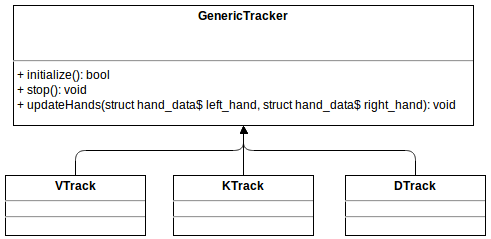
\includegraphics[scale=0.5]{image/ktrack_implement.png}
	\caption{Relations d'héritage entre périphériques de tracking}
\end{figure}

KTrack récupère les données du réseau grâce à la partie client OSC.

\section{Premiers résultats}

Par défaut, le mode de dessin est actif lorsque les deux mains sont jointes, mais cela provoque dans certains angles des erreurs de positions. En effet, lorsqu'une main masque l'autre main, Kinect considère que la main masquée n'existe plus, ce qui renvoie des coordonnées erronées. Pour corriger ce problème, il a été proposé de changer le mode d'activation du dessin.

En plus du problème concernant le déclenchement du mode de dessin, il a été observer que les données recu de la Kinect sont bruitées. Ce bruit a pour résultat un tremblement du curseur et donc une imprécision lors des dessins.

Voici une illustration de l'effet du bruit sur le dessin :


\begin{figure}[!ht]
	\center
	
\includegraphics[scale=0.5]{image/bruit.png}
	\caption{Dessin d'un smiley, bruitage trop important}
\end{figure}

Dessiner une figure est très compliqué avec le bruit comme visible sur le dessin du smiley.
 


\chapter{Analyse du bruit}

Lors de l'utilisation de Kinect, la position du curseur était bruité, celui-ci tremblait. Le bruit est un signal "haute-fréquence" parasite qui se superpose au mouvement du curseur qui est un signal "basse-fréquence". Il faut donc garder uniquement le signal "haute-fréquence".

Pour faire cela, l'utilisation d'un filtre passe-bas est possible. Le filtre passe-bas est un type de filtre qui permet de supprimer les signaux qui dépassent une fréqeunce indiqué et donc de garder uniquement les signaux inférieures à la fréquence voulue. Le désavantage des filtres est qu'ils introduisent une latence, ce qui est génant dans une application de dessin, le dessin n'étant plus effectué en même temps que le déplacement de la main. Le filtre utilisé est le One Euro Filter. C'est un filtre passe-bas developpé par l'INRIA et qui permet d'avoir une fréquence variable. Le filtrage peut donc être plus ou moins important selon le tracé effectué ?

Le filtrage du tracé pouvant provoquer une latence importante, il était nécessaire de trouver un moyen pour prédire la position du point suivant pour pouvoir masquer cette latence.

Le dead reckoning est un algorithme qui permet de calculer une position à partir de la trajectoire actuelle et de la vitesse. Cet algorithme est notamment utilisé dans la navigation navale et aerienne, et dans les jeux-videos en ligne. 


\chapter{One Euro filter}

Le One Euro filter est un algorithme permettant permettant de filtrer un tracé. Nous allons donc nous servir de cet algorithme pour pallier le bruit obtenu dans les données récupérées de la Kinect.

\section{Présentation}
 Le One Euro filter \cite{oneeuro} est un filtre développé par l'INRIA et dont l'implémentation dans certains langages dont le C++ est disponible sur internet. Celui-ci est un filtre passe-bas, c'est à dire que les hautes frequences sont eliminées. Cela permet ainsi d'éliminer les tremblements du curseur.
	
\section{Implémentation}

Une implémentation en C++ du \textit{One Euro Filter} est disponible sur internet.

%le code ou on filtre dans le Ktrack

Il a été décidé de faire le traitement des données coté client et non serveur pour que l'application puisse desactiver le filtrage si nécessaire, et utiliser en paralléle les données filtrées et les données bruitées.
Une fois le filtre utilisé une latence entre le moment où le mouvement est effectué et le déplacement du curseur est apparue. Ceci étant gênant pour une application de dessin, nous avons dù régler les paramètres du One Euro Filter pour réduire cette latence.

\section{Réglage}

Le réglage du One Euro Filter est une partie importante du projet puisqu'elle affecte l'expérience de l'utilisateur. Il nous faut corriger au mieux le signal que l'on reçoit de la Kinect sans pour autant causer une gêne d'utilisation. Nous avons observé les exemples du One Euro Filter \cite{oneeurodemo}, et nous avons modifié nos paramètres de filtre.

Nous avons fait tester l'application par plusieurs personnes et ajuster les paramètres de filtre en fonction de leurs retours d'utilisation.

Nous obtenons finalement une utilisation très fluide et réactive avec un traitement du signal efficace. 

Voici un aperçu du résultat de l'application du filtre:

\begin{figure}[!ht]
	\center
	
\includegraphics[scale=0.6]{image/bruit.png}
	\caption{Dessin d'un smiley, bruitage trop important}
	
\includegraphics[scale=0.6]{image/nonbruit.png}
	\caption{Dessin d'un smiley, bruitage réduit par le filtre}
\end{figure}

Compte-tenu du bruit obtenu par une Kinect, il serait très compliqué d'obtenir un résultat de meilleure qualité sans utiliser des paramètres de lissage plus conséquents, combinés avec des algorithmes de prédiction tels que le dead reckoning.
\chapter{Perspective}
Avant le réglage du filtre, des recherches sur le dead reckoning ont été effectué pour pouvoir masquer la latence si elle persistait.

\section{Dead Reckoning}

Le filtrage du tracé provoquant une latence avant le réglage du filtre, il était nécessaire de trouver un moyen pour prédire la position du point suivant pour pouvoir masquer cette latence au cas où celle-ci serait toujours présente une fois le filtre réglé. C'est dans cette optique que nous avons effectué des recherches sur le dead reckoning.

Le dead reckoning est un algorithme qui permet de calculer une position à partir de la trajectoire actuelle et de la vitesse. Cet algorithme est notamment utilisé dans la navigation navale et aerienne, et dans les jeux-videos en ligne. 
La formule du dead recknoning trouvé et qui est utilisé dans les jeux-videos  est \textit{P$_{t}$ = P$_{0}$ + V$_{0}$T + A$_{0}$*T\up{2}} avec :

\begin{itemize}
	\item P$_{t}$ = position à l'instant T
	\item V$_{0}$ = vitesse au dernier point
	\item T = temps entre deux points
	\item A$_{0}$ = acceleration entre les deux derniers points
\end{itemize}

Toutefois, cette formule est incomplète car elle ne prend pas en compte l'angle d'orientation. Mais la formule compléte et générale n'a pus être trouvé, en effet le dead reckoning est différent selon les données traitées.

Par exemple, dans un jeu de voiture, l'algorithme va prendre en compte la présence d'un virage proche dans le vitesse pour freiner et dans l'angle d'orientation pour commencer à tourner dans la direction.
Aprés avoir paramétré le filtre, la latence est fortement amoindri et est devenu acceptable. A cause de la difficulté de l'implementation du dead recknoning, il a été decidé de ne pas le coder.

\section{Changement du geste de déclenchement du mode dessin}
Lors du déclenchement du mode dessin, effectué en tapant dans les mains, un tracé non desiré d'effectue car OpenNI ne reconstitue pas correctement le squelette, une des mains cachant l'autre. 
Pour régler ce probléme, plusieurs idées ont été soulevées. Tout d'abord, à declencher le mode dessin lorsque le poing est fermé. Mais pour pouvoir effectuer cela, il est nécessaire que la caméra Kinect soit proche de la main ce qui est incompatible avec le dessin pour lequel la caméra doit étre eloigné pour pouvoir dessiner avec une fenetre de dessin dont la dimension en largeur correspond à la distance les bras écartés du corps.
Ensuite , il a été pensé de declencher le dessin cinq secondes aprés la détection du geste de declenchement. Cela permettrait d'enlever le tracé non désiré au début et de laisser la possibilité à l'utilisateur de placer correctement sa main à l'endroit de début de tracé voulue. L'affichage du message se faisant dans le fichier .json correspondant à l'affichage desiré.






%input{DeadReckoning.tex}
\chapter{Conclusion}

Nous avons vu dans ce rapport la phase d'analyse de notre projet. Celui-ci consiste en l'amélioration d'une application de tracking existant permettant le contrôle de la souris. 

Nous avons examiné plusieurs solutions pour corriger le problème de non visualisation de l'espace d'interaction et du manque de retour physique tout en rendant l'application multi-utilisateurs. Pour répondre à ces problèmatiques, nous avons étudié plusieurs solutions telles que l'utilisation d'ARTrack ou d'utiliser plusieurs Kinect. 

Comme nous souhaitions rendre l'application grand public, nous avons préféré opter pour une solution n'utilisant qu'une seule Kinect, celle-ci sera positionnée en hauteur avec un angle spécifique pour permettre d'observer le support sans avoir d'oclusions selon l'angle du support. 

Maintenant que la partie analyse est accomplie, nous allons pouvoir commencer l'implémentation de notre solution. Cependant, il est possible que certaines difficultés apparaissent en cours de projet. Notamment, l'absence de retour d'information concernant la réussite du tracking de l'objet support.
\chapter{Glossaire}

\textbf{Kinect} Il s'agit d'une caméra utilisant des techniques d'interaction développées par la société israélienne PrimeSense, longtemps nommée par le nom de code du projet, "Project Natal", elle a été officialisée juste avant l'E3 sous le nom Kinect. Elle est basée sur un périphérique d'entrée branché sur la console Xbox 360 qui permet d'interagir par commande vocale (pas disponible au lancement en France), reconnaissance de mouvement et d'image.\\

\textbf{Tracking} est l'ensemble des moyens mis en oeuvre pour suivre, dans
notre contexte, un corps en mouvement.\\

\textbf{ARTrack} L’ARTrack (Advanced Realtime Tracking) est un ensemble de caméra infrarouge développé par la société Vicon. Ces caméras fonctionnent gráce a des marqueurs. Il est possible de traquer avec précision n’importe quel élément équipé des trackers.\\

\textbf{QR Code} Les QR Codes sont un type de codes barres à deux dimensions.\\

\textbf{SDK} Un SDK (Software Development Kit) est un ensemble d'outils permettant aux développeurs de créer des applications.
\bibliography{Bibliography}
%%%%%%%%%%%%%%%%%%%%%%%%%%%%%%%%%%%%%%% contenu futur

\newpage
\chapter*{Résumé}

TODO ?


\end{document}